%! Licence = CC BY-NC-SA 4.0

%! Author = gianfluetsch
%! Date = 30. Dez 2021
%! Project = cydef_summary

\section{Windows Logs}

\subsection{TLP (Traffic Light Protocol)}
\begin{itemize}
    \item RED $\rightarrow$ Infos sind auf den \textbf{Kreis der Anwesenden} beschränkt $\rightarrow$ Weitergabe ist untersagt
    \item Amber $\rightarrow$ infos darf der Empfänger \textbf{innerhalb seiner Organisation} aus Basis “Kenntnis \textbf{nur wenn nötig}” weitergeben
    \item Green $\rightarrow$ infos dürfen \textbf{innerhalb der Organisation} und an deren Partner weitergegeben, aber \textbf{nicht veröffentlicht} werden
    \item White (default) $\rightarrow$ abgesehen von \textbf{urheberrechtlichen Aspekten} dürfen die Infos \textbf{ohne Einschränkungen} weitergegeben werden
\end{itemize}

\subsection{Event Log Categories}
\begin{itemize}
    \item \textbf{Security.evtx}
    \begin{itemize}
        \item access control and seucrity information
        \item only written by \textit{LSASS} process
        \item \glqq Security Event Log\grqq is most important for cyber defense
        \item System events, logon, account, privilege used, account management, object access, directory service, process tracking
    \end{itemize}
    \item \textbf{System.evtx}
    \begin{itemize}
        \item windows system events (driver, service, ressources)
    \end{itemize}
    \item \textbf{Application.evtx}
    \begin{itemize}
        \item non system related software events
    \end{itemize}
    \item \textbf{<Custom>.evtx}
    \begin{itemize}
        \item around 150 different custom application logs
    \end{itemize}
\end{itemize}

\subsection{LSASS Process}
\begin{itemize}
    \item responsible for enforcing the security policy on the system
\end{itemize}

\subsection{Logging}
Über eine GPO kann ein Logging-Agent (z.B. der Wazuh-Agent) einfach auf allen gewünschten Servern installiert und konfiguriert werden.
Diesen Agent sollte man so konfigurieren, dass er alle wichtigen und relevanten Logs (z.B. die RDP Logs) ebenfalls an Wazuh weiterleitet.
Danach sind diese Logs auch innerhalb von Wazuh zentral ersichtlich und filterbar.

Dabei werden die Events aus dem EventLog an Wazu weitergeleitet und es kann somit auch nach der \textit{EventID} gefiltert werden.

\subsubsection{EventID 1149}
Successful network authentication (successfully executed an RDP network connection).

Event 1149 is logged when there is a successful RDP logon to the computer. Before Windows 7 and Windows Server 2012, 1149 would be logged for any initiation of an RDP connection, so it was not a useful indicator for an actual successful application of user credentials.

But, that has changed, and all modern OS versions will only log 1149 if the username in the event was successfully authenticated. It also includes the IP address of the source of the connection, which is useful information. If an account is used and successfully authenticates but does not have
permission to RDP to the computer due to other restrictions, event 1149 is not generated.


\subsubsection{Phases of RDP-Connection}

\begin{minipage}{0.45\linewidth}
    \begin{enumerate}
        \item Connection Initiation
        \item Basic Settings Exchange
        \item Channel Connection
        \item RDP Security Commencement
        \item Secure Settings Exchange
        \item Optional Connect-Time Auto-Detection
        \item Licensing
        \item Optional Multitransport Bootstrapping
        \item Capabilities Exchange
        \item Connection Finalization
    \end{enumerate}
\end{minipage}
\begin{minipage}{0.5\linewidth}
    \begin{center}
        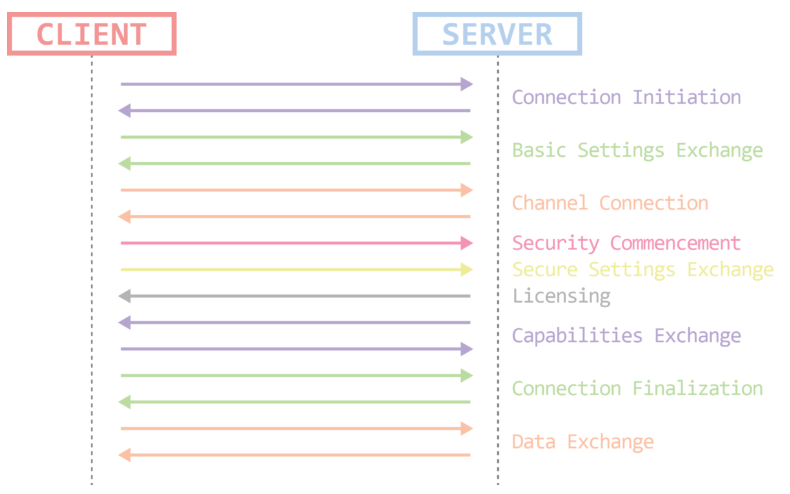
\includegraphics[width=1.2\linewidth]{img/rdp_phases}
        \vspace{-8pt}
    \end{center}
\end{minipage}

\subsubsection{Explain how you filtered every RDP login attempt}
The TerminalServices-RemoteConnectionManager Log is not forwarded to Wazuh.\\
Unable to filter for all the attempts.
With the current Wazu setup, one must filter for Logon Type 3 \& 10 (remote logon types)\\

\begin{itemize}
    \item \lstinline|data.win.system.eventID = 4624| or \lstinline|data.win.system.eventID = 4625|
    \item \lstinline|data.win.sytem.eventID: 4624| and \lstinline|data.win.evendata.logonType: 3|
\end{itemize}

\subsubsection{Explain how you filtered unsuccessful RDP login attempts}
Um erfolglose RDP Login Versuche im Event Viewer zu suchen, sucht man nach der \lstinline|Event ID: 4625|.\\

\begin{itemize}
    \item \lstinline|data.win.eventdata.logonType = 3| or \lstinline|data.win.eventdata.logonType = 10|
    \item \lstinline|data.win.system.eventID = 4625| and \lstinline|data.win.eventdata.logonType = 3|
\end{itemize}